\section{Dilemmas and Trilemmas\label{sec:dilemma_trilemma}}

% Not included here: 
% https://en.wikipedia.org/wiki/The_Innovator%27s_Dilemma
% because it is the etic view of change



When a decision has two viable options (neither being best), that presents a \href{https://en.wikipedia.org/wiki/Dilemma}{dilemma}. The name for the case with three viable options is a \href{https://en.wikipedia.org/wiki/Trilemma}{trilemma}. 

% claim
Dilemmas explain the inherent complexity of bureaucracy even when bureaucrats are honest and the purpose of the organization is clear.
% relevance
The point isn't that one should select one of the two options. The point of a dilemma is that it is a marker that there is a decision to be made.
% consequence
The action for the bureaucrat in response to this assessment is to talk with fellow bureaucrats about these dilemmas. Rather than seeking consensus, strive for comprehension of other people's perspective. That way you can navigate processes more effectively.

\subsection{How Dilemmas arise in bureaucracy}

Given a task, the simplest response for an individual is to take action and be done. 

If the task is more challenging, it may be necessary to first make a plan, then take action and be done. The source of the challenge may be task complexity, scale, number of people impacted, diversity of stakeholders, amount of time needed, how the current task shapes future decisions, number of collaborators, etc. Regardless of why the task is challenging, a dilemma has already arisen: how much time to spend planning versus doing. 

If the task is even more challenging, it may be useful to gather data for the plan, then make a plan, then take action and be done. A new dilemma arises: how much time to spend gathering data versus planning. The previous dilemma still exists -- planning versus doing. As an alternative to the dilemma framing, how much time should be allocated to three categories of activity?

But wait, how did the person in the first scenario (just do the task) know no plan was necessary? Either it was an explicit choice or they didn't perceive the need to decide about whether to plan. Someone else faced with that same task might choose differently, e.g., to make a plan. The task complexity is relative to the person's skills, experiences, and expectations about stakeholders and ramifications.

In this escalating sequence of increasingly challenging tasks, suppose the task involves you and another person. The overhead of coordination inflicts additional dilemmas. 

An independent source of friction is when people involved in the task don't agree on how challenging it is. The framing of the difficulty matters because it alters how much time is left for carrying out the action. 

The choice of ``how complicated is the task?'' shapes the team dynamics and hierarchical roles. 

\subsection{Folk wisdom on decision making in the face of dilemmas}

\href{https://en.wikipedia.org/wiki/Hick\%27s_law}{Hick's law}\marginpar{[Tag] Folk wisdom}: ``increasing the number of choices will increase the decision time logarithmically.''

\href{https://en.wikipedia.org/wiki/Hanlon\%27s_razor}{Hanlon's razor}\marginpar{[Tag] Folk wisdom}: ``never attribute to malice that which is adequately explained by stupidity.''

\href{https://en.wikipedia.org/wiki/Parkinson\%27s_law}{Parkinson's law}\marginpar{[Tag] Folk wisdom}: ``work expands so as to fill the time available for its completion.''

\href{https://en.wikipedia.org/wiki/Murphy\%27s_law}{Murphy's law}\marginpar{[Tag] Folk wisdom}: ``Anything that can go wrong will go wrong.''

\href{https://en.wikipedia.org/wiki/Law_of_triviality}{Law of Triviality}\marginpar{[Tag] Folk wisdom}: ``people within an organization commonly or typically give disproportionate weight to trivial issues.''


\subsection{Dilemmas are a poor framing}

Although the following concepts are presented as dilemmas and trilemmas, these are necessarily simplifications. For example, two ways to simplify situations into a dilemma are
\begin{itemize}
    \item start with a single variable, e.g., "how much data gathering", and force it into a binary choice "more data gathering" versus "less data gathering"
    
    % a reduction of a complicated situation to one variable. 
    \item start with a complex trade-off space with many opportunities and reduce it to a false dichotomy of zero-sum options: "more data gathering" vs "more planning." The actual trade-space involves optimization of multiple objectives, like (maximize productivity) and (minimize risk) and (maximize quality) and (maximize employee satisfaction) and (minimize latency). 
    % https://bennorthrop.com/Essays/2022/code-ownership-stewardship-or-free-for-all.php
\end{itemize}
These over-simplifications neglect both the continuous nature of the trade-offs and the alternative creative approaches to a specific situation. 

\subsection{Dilemmas as a framing to ease you into the complexity}
The choices are described here in simplified representation as a starting point intended to introduce the decision space relevant to individual bureaucrats. Awareness of these dilemmas and trilemmas are intended to spark creative imagination about the nuances specific to your situation.

Do not accept the dilemmas presented here as the final framing. Thinking in terms of a limited spectrum of opportunities neglects nuances that enable more creative approaches. Ponder theses dilemmas prior to the pressure of real-time decision making.  Recognize dilemmas and trilemmas and then avoid them by adapting to the local conditions and specific people available to help.

\subsection{Dilemmas are not purely intellectual}
Decision making is not a purely intellectual task; there is emotional stress induced by the process. Dilemmas create cognitive dissonance for the decision maker. Any selection is going to have downsides, and any compromise will be suboptimal. Those burdens weigh on deciders.

\subsection{Additional complications}
Adding to the difficulty and stress, dilemmas presented here are occur concurrently and continuously. The dilemmas are inter-dependent due to both to the common variables and the constrained resources.
Selecting an option for one dilemma alters the options available in other dilemmas.

Oscillation between approaches can be caused by change of management, accumulation of experience (dissatisfaction) with one solution, the desire for promotion (change as progress), desire for cost savings. The rate of oscillation is an indicator of the half-life of institutional memory. 


\subsection{Personal Policies}

In practice, the following decisions are unordered and are constantly faced by the bureaucrat. As observed in \cite{1959_Lindblom}, this flurry of decisions contrasts to a regularized process that might be envisioned as optimal.


Suppose you learn of something prior to official deployment (i.e., you learn of the internal musings of another team).  
\begin{center}
\begin{table}[ht]
\begin{tabular}{ | m{\dilemmatablewidth}| m{\dilemmatablewidth} | } 
  \hline
  \textbf{Intervene before the deployment of a policy or process or product, perhaps without relevant context.} &
  \textbf{Wait with feedback until deployment.} \\
  \hline
  \textit{Cons}: engaging prematurely betrays your awareness, so future explorations become more silo'd. & 
  \textit{Cons}: the team wasted time and attention on something that wouldn't work or may even be harmful. \\
  \hline
\end{tabular}
\caption{dilemma of early intervention. See the related dilemma of micromanaging.}
\label{table:early-intervention}
\end{table}
\end{center}

\begin{center}
\begin{table}[ht]
\begin{tabular}{ | m{\dilemmatablewidth}| m{\dilemmatablewidth} | } 
  \hline
  \textbf{Review status of the work of other people early and often.} &
  \textbf{Review status infrequently.} \\
  \hline
  \textit{Description}: Micromanagement. & 
  \textit{Description}: Hands-off management style. \\
  \hline
  \textit{Cons}: Takes up your time and the people you're reviewing. & 
  \textit{Cons}: . \\
  \hline
\end{tabular}
\caption{dilemma of micromanaging.}
\label{table:micromanaging}
\end{table}
\end{center}

\begin{center}
\begin{table}[ht]
\begin{tabular}{ | m{\dilemmatablewidth}| m{\dilemmatablewidth} | } 
  \hline
  \textbf{Write everything down to cover your ass.} &
  \textbf{Don't record sensitive conversations that could be used against you.} \\
  \hline
  \textit{Cons}: Takes a lot of time and effort to accurately capture intent. Recording can be done poorly or be misconstrued.  & 
  \textit{Cons}: No written record to point to when someone changes their behavior. \\
  \hline
\end{tabular}
\caption{There are many dark patterns in this trade-off.}
\label{table:notes_or_no_notes}
\end{table}
\end{center}


\begin{center}
\begin{table}[ht]
\begin{tabular}{ | m{\dilemmatablewidth}| m{\dilemmatablewidth} | } 
  \hline
  \textbf{Ponder what should or could be done.} &
  \textbf{Figure out how to accomplish the objective.}\\
  \hline
  \textit{Cons}: . & 
  \textit{Cons}: . \\
  \hline
\end{tabular}
\caption{How much time to spend admiring the trees versus the forest. 
}
\label{table:forest-vs-trees}
\end{table}
\end{center}




\begin{center}
\begin{table}[ht]
\begin{tabular}{ | m{\dilemmatablewidth}| m{\dilemmatablewidth} | } 
  \hline
  \textbf{how much time to allocate for meetings to facilitate coordination} &
  \textbf{how much time for action} \\
  \hline
  \textit{Description}: . &
  \textit{Description}: . \\
  \hline
  \textit{Cons}: . & 
  \textit{Cons}: . \\
  \hline
\end{tabular}
\caption{
}
\label{table:meetings-versus-work}
\end{table}
\end{center}


\begin{center}
\begin{table}[ht]
\begin{tabular}{ | m{\dilemmatablewidth}| m{\dilemmatablewidth} | } 
  \hline
  \textbf{Operate at the level you are being paid for.} &
  \textbf{Operate above the level that you are being paid for in order to be a promoted.} \\
  \hline
  \textit{Description}: Meet job requirements but nothing extra. &
  \textit{Description}: Exceed job requirements. \\
  \hline
  \textit{Cons}: risk not being promoted. & 
  \textit{Cons}: experience wage loss - Organization is getting free labor \\
  \hline
\end{tabular}
\caption{Work above your pay grade (extra labor, reduced pay) or at your pay grade (expected labor and pay)?
}
\label{table:work_extra_or_work_as_expected}
\end{table}
\end{center}


\begin{center}
\begin{table}[ht]
\begin{tabular}{ | m{\dilemmatablewidth}| m{\dilemmatablewidth} | } 
  \hline
  \textbf{speak out/speak up.} &
  \textbf{hold back comments and questions.} \\
  \hline
  \textit{Cons}: . & 
  \textit{Cons}:  \\
  \hline
\end{tabular}
\caption{
}
\label{table:speak-up-or-hold-back}
\end{table}
\end{center}


\begin{center}
\begin{table}[ht]
\begin{tabular}{ | m{\dilemmatablewidth}| m{\dilemmatablewidth} | } 
  \hline
  \textbf{Send bad news up the chain of command} &
  \textbf{Minimize bad news up the chain of command} \\
  \hline
  \textit{Pros}: Reliable source of news. &
  \textit{Pros}: Minimize burden of management. \\
  \hline
  \textit{Cons}: You are viewed as a source of problems. & 
  \textit{Cons}: Harmful events eventually catch up with the org.  \\
  \hline
\end{tabular}
\caption{Example: Challenger disaster.}
\label{table:bad-news-up-the-chain}
\end{table}
\end{center}



\begin{center}
\begin{table}[ht]
\begin{tabular}{ | m{\dilemmatablewidth}| m{\dilemmatablewidth} | } 
  \hline
  \textbf{Prepare for disasters and emergencies, invest in mitigation} &
  \textbf{Wait for the problem to arise} \\
  \hline
  \textit{Pros}: Lessen the impact when bad things happen; decrease the number of problems from occurring in the first place. &
  \textit{Pros}: deal with the specifics of the scenario at that time and thus be better informed. \\
  \hline
  \textit{Cons}: fewer events evolve into emergencies because you're prepared, or the impact of disasters is lessened. Both make you look overly paranoid and wasteful. & 
  \textit{Cons}: Unexpected events result in worse outcomes.  \\
  \hline
\end{tabular}
\caption{How much to invest in contingency planning and preparedness.}
\label{table:emergencies-vs-ignore}
\end{table}
\end{center}

% https://graphthinking.blogspot.com/2019/08/two-misleading-simplifications-when.html
\begin{center}
\begin{table}[ht]
\begin{tabular}{ | m{\dilemmatablewidth}| m{\dilemmatablewidth} | } 
  \hline
  \textbf{Focus on the problem at hand} &
  \textbf{Ponder the systemic issues} \\
  \hline
  \textit{Description}: Focus on isolated problematic aspects and do not account for the interdependencies and feedback loops and stakeholder incentives. &
  \textit{Description}: Philosophical musings. \\
  \hline
  \textit{Cons}: This simplification is misleading because Emergent behavior can not be tackled by inspecting components in isolation. & 
  \textit{Cons}: \\
  \hline
\end{tabular}
\caption{
}
\label{table:focus-vs-systemic}
\end{table}
\end{center}

\begin{center}
\begin{table}[ht]
\begin{tabular}{ | m{\dilemmatablewidth}| m{\dilemmatablewidth} | } 
  \hline
  \textbf{seek recognition} &
  \textbf{work in obscurity} \\
  \hline
  \textit{Pros}: . & 
  \textit{Pros}: . \\
  \hline
  \textit{Cons}: . & 
  \textit{Cons}: . \\
  \hline
\end{tabular}
\caption{
}
\label{table:recognition-obscurity}
\end{table}
\end{center}

\begin{center}
\begin{table}[ht]
\begin{tabular}{ | m{\dilemmatablewidth}| m{\dilemmatablewidth} | } 
  \hline
  \textbf{only let good ideas through (based on a detailed review process of clearly specified plan)} &
  \textbf{give resources to untested ideas, some of which will fail} \\
  \hline
  \textit{Pros}: . & 
  \textit{Pros}: . \\
  \hline
  \textit{Cons}: . & 
  \textit{Cons}: . \\
  \hline
\end{tabular}
\caption{
}
\label{table:idea-filtering}
\end{table}
\end{center}


% https://graphthinking.blogspot.com/2016/06/innovation-in-open-versus-behind-curtain.html
\begin{center}
\begin{table}[ht]
\begin{tabular}{ | m{\dilemmatablewidth}| m{\dilemmatablewidth} | } 
  \hline
  \textbf{work on disruptive innovation in the open} &
  \textbf{work on disruptive innovation in hiding} \\
  \hline
  \textit{Description}:  &
  \textit{Description}: .  \\  
  \hline
  \textit{Pros}: more likely to be criticized. Criticism can be positive (as in an incubator setting) or .. & 
  \textit{Pros}: less drama -- the incumbent won't attack the innovation since they don't know about it. \\
  \hline
  \textit{Cons}: negative Criticism intended to harm -- an incumbent has reason to be defensive. The incumbent attacks the innovation before it is sufficiently developed or has time to build a user base. & 
  \textit{Cons}: less opportunity for feedback. \\
  \hline
\end{tabular}
\caption{
}
\label{table:innovate-open-obscure}
\end{table}
\end{center}

% https://graphthinking.blogspot.com/2016/05/claim-innovation-is-either-disruptive.html
\begin{center}
\begin{table}[ht]
\begin{tabular}{ | m{\dilemmatablewidth}| m{\dilemmatablewidth} | } 
  \hline
  \textbf{disruptive innovation} &
  \textbf{iterative (evoluationary) innovation} \\
  \hline
  \textit{Description}:   &
  \textit{Description}: starts with change to existing solution.  \\  
  \hline
  \textit{Pros}: high reward. & 
  \textit{Pros}: low risk, low cost. \\
  \hline
  \textit{Cons}: high risk, high cost. & 
  \textit{Cons}: low reward. \\
  \hline
\end{tabular}
\caption{
}
\label{table:disruptive-or-iterative}
\end{table}
\end{center}

\begin{center}
\begin{table}[ht]
\begin{tabular}{ | m{\dilemmatablewidth}| m{\dilemmatablewidth} | } 
  \hline
  \textbf{Gather lots of data} &
  \textbf{Gather minimal data} \\
  \hline
  \textit{Description}: Gather lots of data for a well-informed decision &
  \textit{Description}: Minimal information because decision maker knows what to do or outcome is irrelevant.  \\  
  \hline
  \textit{Cons}: High cost of gathering data (time, resources). \href{https://en.wikipedia.org/wiki/Opportunity_cost}{Opportunity costs}. & 
  \textit{Cons}: Lack of data results in decisions based on oversimplified assessment \\
  \hline
\end{tabular}
\caption{How much data to gather for a decision. See Fig.~\ref{fig:data_collection_cost_uncertainty}. See also \S~\ref{sec:bureaucratic_debt} on bureaucratic debt.
%{\tiny Tag: Decision making.}
}
\label{table:gather_data_lots-vs-little}
\end{table}
\end{center}

\begin{figure}[ht]
        \centering
        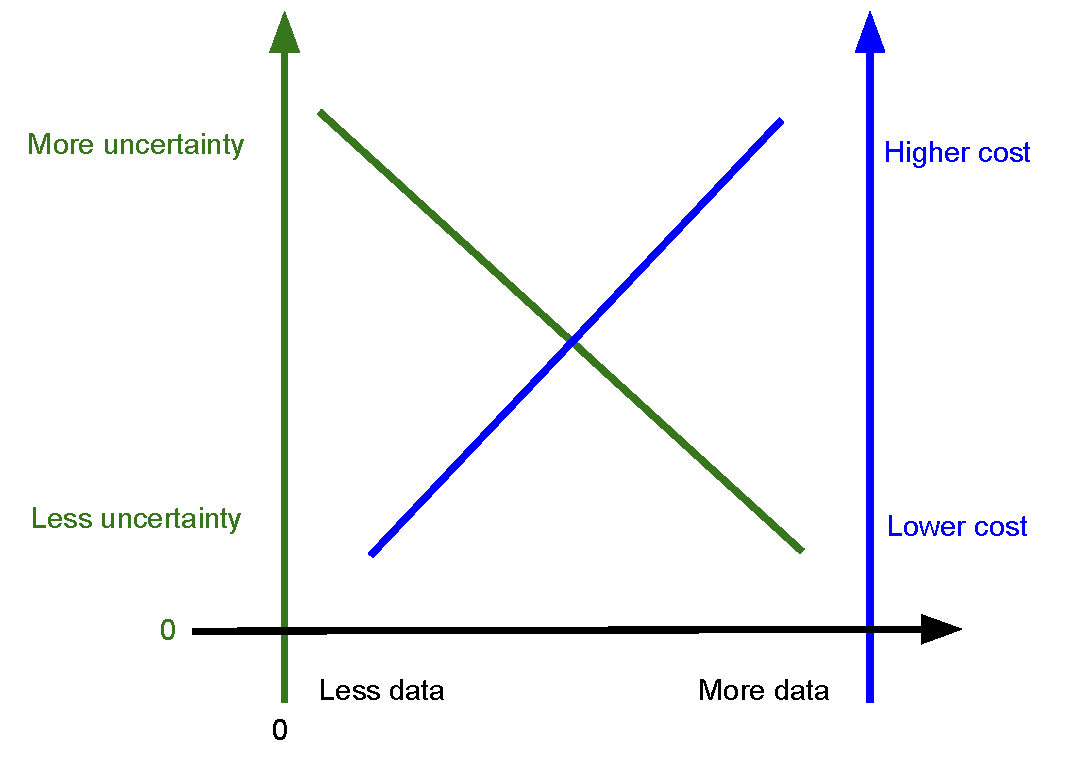
\includegraphics[width=0.8\textwidth]{images/cost_and_uncertainty_for_data_collection}
        \caption{Collecting more data costs money and decrease uncertainty. See Dilemma~\ref{table:gather_data_lots-vs-little}.}
        \label{fig:data_collection_cost_uncertainty}
\end{figure}

The logistics of gathering data can be measured, but there are other subjective aspects to account for as well. Making a decision has an emotional toll on the decider due to the risk of failure. Also, decisions are made in a social context, with decision makers accounting for the ramifications on people they have relationships with. 


Gathering data (Dilemma~\ref{table:gather_data_lots-vs-little}) is distinct from planning (Dilemma~\ref{table:planning}). It is possible to do a lot of planning with only a little information gathered, and it is feasible to have lots of data and do no planning. 

\begin{center}
\begin{table}[ht]
\begin{tabular}{ | m{\dilemmatablewidth}| m{\dilemmatablewidth} | } 
  \hline
  \textbf{Extensive planning upfront (proactive)} & 
  \textbf{Iterative improvement of plans (reactive)} \\ 
  \hline
  \textit{Description}: Lots of time spent brainstorming potential scenarios and contingency options prior to taking action. & 
  \textit{Description}: Start taking action and use feedback to shape next actions. \\ 
  \hline
  \textit{Cons}: ``No plan survives contact with the enemy.'' & 
  \textit{Cons}: Less prepared. \\  
  \hline
\end{tabular}
\caption{How much time to invest in planning
%{\tiny Tag: Decision making.}
}
\label{table:planning}
\end{table}
\end{center}

\begin{center}
\begin{table}[ht]
\begin{tabular}{ | m{\dilemmatablewidth}| m{\dilemmatablewidth} | } 
  \hline
  \textbf{plans that involve many milestones/check-ins/updates} &
  \textbf{plan to just do it} \\
  \hline
  \textit{Description}: . & 
  \textit{Description}: . \\ 
  \hline
  \textit{Cons}:  & 
  \textit{Cons}: . \\  
  \hline
\end{tabular}
\caption{Engagement with opposition to process or change.
%{\tiny Tag: Decision making.}
}
\label{table:just-do-it}
\end{table}
\end{center}


\begin{center}
\begin{table}[ht]
\begin{tabular}{ | m{\dilemmatablewidth}| m{\dilemmatablewidth} | } 
  \hline
  \textbf{Involve people who disagree} & 
  \textbf{Ignore people who disagree} \\ 
  \hline
  \textit{Description}: . & 
  \textit{Description}: . \\ 
  \hline
  \textit{Cons}:  & 
  \textit{Cons}: . \\  
  \hline
\end{tabular}
\caption{Engagement with opposition to process or change.
%{\tiny Tag: Decision making.}
}
\label{table:opposition}
\end{table}
\end{center}

Making a decision imposes a bound on how much time is available for both gathering data and planning. Time is zero sum, so more time gathering data is less time planning. Similarly, the number of people available for data gathering and planning is bounded, and tasking people is a zero sum choice.

\begin{figure}[ht]
    \centering
    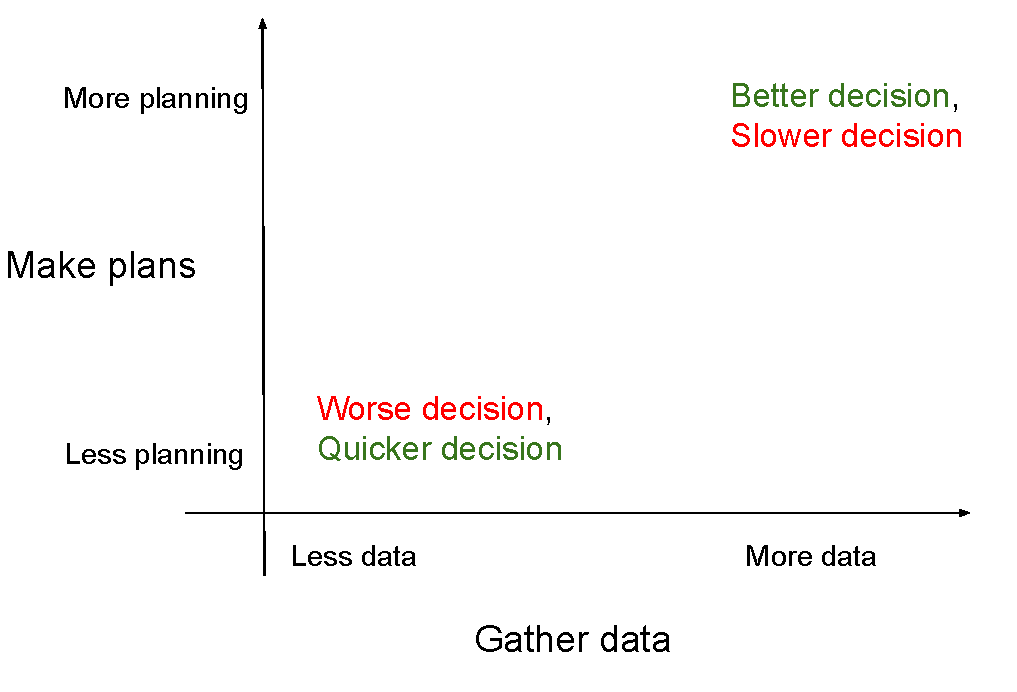
\includegraphics[width=0.8\textwidth]{images/planning_and_data_gathering.pdf}
    \caption{Planning (Dilemma~\ref{table:planning}) and data gathering (Dilemma~\ref{table:gather_data_lots-vs-little}) trade-off.}
    \label{fig:pareto_frontier}
\end{figure}

Practically, gathering data and planning never terminate, they evolve 




When planning (Dilemma~\ref{table:planning}), aspects to consider include
\begin{itemize}
    \item the amount of risk seeking or tolerance (Dilemma~\ref{table:risk})
    \item intended scope of impact -- Dilemma~\ref{table:scope_broad-vs-narrow}
\end{itemize}

\begin{center}
\begin{table}[ht]
\begin{tabular}{ | m{\dilemmatablewidth}| m{\dilemmatablewidth} | } 
  \hline
  \textbf{Take on big risks and big rewards} & 
  \textbf{Take on small risks and small rewards} \\ 
  \hline
  \textit{Description}: high risk tolerance &
  \textit{Description}: low risk tolerance \\
  \hline
  \textit{Pros}: Potential for failure and harm is significant &
  \textit{Pros}: If any one investment fails, you can continue other efforts. \\
  \hline
  \textit{Cons}:  & 
  \textit{Cons}: Incremental can be slower. \\
  \hline
\end{tabular}
\caption{Risk tolerance. 
%{\tiny Tag: Personal choice.}
}
\label{table:risk}
\end{table}
\end{center}

\ \\

\begin{center}
\begin{table}[ht]
\begin{tabular}{ | m{\dilemmatablewidth}| m{\dilemmatablewidth} | } 
  \hline
  \textbf{Broad scope of impact} &
  \textbf{Narrow scope of impact} \\
  \hline
  \textit{Description}: The consequence of the work has many stakeholders &
  \textit{Description}: Small number of stakeholders \\  
  \hline
  \textit{Pros}:  &
  \textit{Pros}: Niche impact means less dependencies on other people. \\
  \hline
  \textit{Cons}: Harder to get everyone in agreement. & 
  \textit{Cons}: Less visibility to the rest of the organization. \\
  \hline
\end{tabular}
\caption{Scope of impact of your work. 
%{\tiny Tag: Personal choice}
}
\end{table}
\label{table:scope_broad-vs-narrow}
\end{center}


Once data is gathered (Dilemma~\ref{table:gather_data_lots-vs-little}) and a plan is made (Dilemma~\ref{table:planning}), the result is disseminated. The choice on how to disseminate is Dilemma~\ref{table:consistency} and Dilemma~\ref{table:disseminate_one-by-one}.

\begin{center}
\begin{table}[ht]
\begin{tabular}{ | m{\dilemmatablewidth}| m{\dilemmatablewidth} | } 
  \hline
  \textbf{Guidance updated frequently; Incremental change} & 
  \textbf{Consistent application of policy over time. Rules persist; then sudden drastic change} \\ 
  \hline
  \textit{Pros}: Adapt policy to new information and changing conditions. &
  \textit{Pros}: Stability is easier to predict between regime changes.  \\
  \hline
  \textit{Cons}: More work needed. Accused of lacking stability. & 
  \textit{Cons}: Doesn't adapt as conditions change. Accused of being inflexible to evolving conditions. \\
  \hline
\end{tabular}
\caption{Consistency over time. Stability of rules; how change is implemented. Can also be characterized as when to tell other people: sooner or later (when firmer information is available) See \S~\ref{sec:static-dynamic_processes} for static versus dynamic processes.
%{\tiny Tag: Organization's culture. Tag: Personal choice.}
}
\label{table:consistency}
\end{table}
\end{center}

Deployment of products and deployment of policies face similar dilemmas. \href{https://en.wikipedia.org/wiki/Diffusion_of_innovations}{Diffusion of Innovation}

\begin{center}
\begin{table}[ht]
\begin{tabular}{ | m{\dilemmatablewidth}| m{\dilemmatablewidth} | } 
  \hline
  \textbf{Tell people one-by-one} & 
  \textbf{Tell everyone at once} \\ 
  \hline
  \textit{Pros}: One on one allows a freer response from audience &
  \textit{Pros}: save time for the speaker. \\
  \hline
  \textit{Cons}: Order matters. & 
  \textit{Cons}: . \\  
  \hline
\end{tabular}
\caption{How to disseminate information
%{\tiny Tag: Personal choice.}
}
\label{table:disseminate_one-by-one}
\end{table}
\end{center}

Once a decision has been made, the decision is executed or enforced. How many rules are there (Dilemma~\ref{table:number_of_rules}) and
how strictly are the rules enforced (Dilemma~\ref{table:rule_strictness})?

\begin{center}
\begin{table}[ht]
\begin{tabular}{ | m{\dilemmatablewidth}| m{\dilemmatablewidth} | } 
  \hline
  \textbf{Enforce rules strictly.} & 
  \textbf{Lax rule enforcement.} \\ 
  \hline
  \textit{Pros}: Predictable &
  \textit{Pros}: Bureaucrats feel empowered. \\
  \hline
  \textit{Cons}: Insensitive to nuance. & 
  \textit{Cons}: Tolerance for changing conditions or exceptional cases.  \\  
  \hline
\end{tabular}
\caption{Strictness of rules.
%{\tiny Tag: Organization's culture.}
}
\label{table:rule_strictness}
\end{table}
\end{center}

\begin{center}
\begin{table}[ht]
\begin{tabular}{ | m{\dilemmatablewidth}| m{\dilemmatablewidth} | } 
  \hline
  \textbf{If it's not against the rules, it must be okay.} & 
  \textbf{I can only do what is allowed by the rules and nothing more.} \\ 
  \hline
  \textit{Pros}: Autonomy &
  \textit{Pros}:  \\
  \hline
  \textit{Cons}: . & 
  \textit{Cons}: .  \\  
  \hline
\end{tabular}
\caption{Adherence to rules.
}
\label{table:rule_adherence}
\end{table}
\end{center}





\begin{center}
\begin{table}[ht]
\begin{tabular}{ | m{\dilemmatablewidth}| m{\dilemmatablewidth} | } 
  \hline
  \textbf{Control via rules} & \textbf{Freedom/autonomy/agility} \\ 
  \hline
  \textit{Description}: high number of rules to cover a variety of situations & 
  \textit{Description}: low number of rules to enable flexibility \\ 
  \hline
  \textit{Cons}: The more rules that exist the more likely it is that someone will find a way to exploit them to their own advantage. & 
  \textit{Cons}: The fewer rules that exist the more likely it is that someone will try to get away with something bad. \\  
  \hline
\end{tabular}
\caption{Number of rules.
%{\tiny Tag: Organization's culture}
}
\label{table:number_of_rules}
\end{table}
\end{center}
Alternative approach: guidance derived from principles that can be adapted to specific situations. That has the problem of requiring good knowledge of the situation and wise judgement.

\ \\

\begin{center}
\begin{table}[ht]
\begin{tabular}{ | m{\dilemmatablewidth}| m{\dilemmatablewidth} | } 
  \hline
  \textbf{I can only do what is legally mandated} & 
  \textbf{I can do anything that's not indicated to be illegal} \\ 
  \hline
  \textit{Description}:  &
  \textit{Description}:  \\
  \hline
  \textit{Pros}:  &
  \textit{Pros}:  \\
  \hline
  \textit{Cons}:  &
  \textit{Cons}:  \\  
  \hline
\end{tabular}
\caption{
}
\label{table:legality}
\end{table}
\end{center}


\begin{center}
\begin{table}[ht]
\begin{tabular}{ | m{\dilemmatablewidth}| m{\dilemmatablewidth} | } 
  \hline
  \textbf{Quickly complete tasks} & 
  \textbf{Methodically complete tasks} \\ 
  \hline
  \textit{Description}: implementing a solution quickly to address urgent needs &
  \textit{Description}: Methodical well-planned design and execution yield robust solutions. \\
  \hline
  \textit{Pros}: rapid solution &
  \textit{Pros}: more like to get the solution right \\
  \hline
  \textit{Cons}: Risk of quick task is that the result is ineffective, inefficient, or wrong &
  \textit{Cons}: \href{https://en.wikipedia.org/wiki/Opportunity_cost}{opportunity cost} \\  
  \hline
\end{tabular}
\caption{Speed versus accuracy of task completion.
}
\label{table:quick-methodical}
\end{table}
\end{center}

\ \\

\begin{center}
\begin{table}[ht]
\begin{tabular}{ | m{\dilemmatablewidth}| m{\dilemmatablewidth} | } 
  \hline
  \textbf{Push people to work really hard} & 
  \textbf{Create a comfortable work environment} \\ 
  \hline
  \textit{Cons}: burn out and leave. & 
  \textit{Cons}: lower instantaneous productivity. \\  
  \hline
\end{tabular}
\caption{Policy enforcement rate
}
\label{table:rate-of-work}
\end{table}
\end{center}

\ \\

% https://bennorthrop.com/Essays/2022/code-ownership-stewardship-or-free-for-all.php
\begin{center}
\begin{table}[ht]
\begin{tabular}{ | m{\dilemmatablewidth}| m{\dilemmatablewidth} | } 
  \hline
  \textbf{One person or team owns an area of responsibility} & 
  \textbf{Anyone take on any task} \\ 
  \hline
  \textit{Cons}: staffing capacity may not be as flexible as varying workload. & 
  \textit{Cons}: not everyone is skilled at everything. \\  
  \hline
\end{tabular}
\caption{Swimlanes, task boundaries.
}
\label{table:swimlanes}
\end{table}
\end{center}

\ \\

\begin{center}
\begin{table}[ht]
\begin{tabular}{ | m{\dilemmatablewidth}| m{\dilemmatablewidth} | } 
  \hline
  \textbf{I expect my management to provide solutions -- just tell me what to do} & 
  \textbf{management is micromanaging -- telling me what to do} \\ 
  \hline
  \textit{Cons}: . &
  \textit{Cons}:  \\  
  \hline
\end{tabular}
\caption{.
}
\label{table:solution_provider}
\end{table}
\end{center}


\ \\

\begin{center}
\begin{table}[ht]
\begin{tabular}{ | m{\dilemmatablewidth}| m{\dilemmatablewidth} | } 
  \hline
  \textbf{seek out experienced collaborators who are probably busy} & 
  \textbf{work with less experienced people who are less set in their ways and opens in more novelty} \\ 
  \hline
  \textit{Cons}: . &
  \textit{Cons}:  \\  
  \hline
\end{tabular}
\caption{.
}
\label{table:experience}
\end{table}
\end{center}


\ \\

\begin{center}
\begin{table}[ht]
\begin{tabular}{ | m{\dilemmatablewidth}| m{\dilemmatablewidth} | } 
  \hline
  \textbf{Say yes to new opportunities} & 
  \textbf{Say no to new opportunities} \\ 
  \hline
  \textit{Pros}: Positive attitude, collaborative. &
  \textit{Pros}: Able to prioritize and focus. \\
  \hline
  \textit{Cons}: Fail to complete tasks. &
  \textit{Cons}: Not a team player \\  
  \hline
\end{tabular}
\caption{Acceptance or rejection of additional work.
}
\label{table:new-opportunties}
\end{table}
\end{center}

\ \\

\begin{center}
\begin{table}[ht]
\begin{tabular}{ | m{\dilemmatablewidth}| m{\dilemmatablewidth} | } 
  \hline
  \textbf{Share less data} &
  \textbf{Share more data} \\
  \hline
  \textit{Description}:  &
  \textit{Description}:  \\  
  \hline
  \textit{Pros}: Restricting data access saves money for the data owner and improves flexibility.&
  \textit{Pros}: Sharing data improves transparency and accountability. \\
  \hline
  \textit{Cons}: Other people (inside and outside the organization) are unable to extract maximum value from data & 
  \textit{Cons}: Sharing data cost resources (people, money, time) \\
  \hline
\end{tabular}
\caption{How much data to share.
%{\tiny Tag: Personal choice.}
}
\label{table:data_share-vs-hide}
\end{table}
\end{center}

\ \\

\begin{center}
\begin{table}[ht]
\begin{tabular}{ | m{\dilemmatablewidth}| m{\dilemmatablewidth} | } 
  \hline
  \textbf{Compete for resources} &
  \textbf{Cooperate for productivity} \\
  \hline
  \textit{Description}: individuals compete for attention and promotion; teams compete for money and staffing resources &
  \textit{Description}: cooperation improves productivity \\  
  \hline
  \textit{Cons}: Fail to synergize skills resources & 
  \textit{Cons}: Not clear who to assign responsibility for success or failure \\
  \hline
\end{tabular}
\caption{Cooperate or Compete -- applies to teams and to individuals. 
%{\tiny Tag: Personal choice.}
}
\label{table:cooperate-vs-compete}
\end{table}
\end{center}

\ \\

\begin{center}
\begin{table}[ht]
\begin{tabular}{ | m{\dilemmatablewidth}| m{\dilemmatablewidth} | }
  \hline
  \textbf{Consistent application of policy across cases} &
  \textbf{adapt policy to specific cases} \\
  \hline
  \textit{Description}: maximize broad applicability; minimize exceptions &
  \textit{Description}:  \\  
  \hline
  \textit{Cons}: Less sensitive to the nuances of a specific situation. & 
  \textit{Cons}: Takes more work. More likely to be accused of bias. \\
  \hline
\end{tabular}
\caption{Case consistency vs adaptability.
%{\tiny Tag: Personal choice.}
}
\label{table:policy_consistency_across_cases}
\end{table}
\end{center}

When change to policies is desired, there are options on how to advocate for change -- Dilemma~\ref{table:how_to_change} 

\begin{center}
\begin{table}[ht]
\begin{tabular}{ | m{\dilemmatablewidth}| m{\dilemmatablewidth} | } 
  \hline
% https://graphthinking.blogspot.com/2019/07/not-too-loose-not-too-tight-determining.html
  \textbf{Adhere strictly to the scope of your role.} & 
  \textbf{Stray outside (or outright ignore) the scope of your role.} \\ 
  \hline
  \textit{Description}: Inflexible to novelty. Specialization of tasking. & 
  \textit{Description}: Lack of structure. Generalization. \\ 
  \hline
  \textit{Cons}: efficiencies of cooperation and specialization would not occur. & 
  \textit{Cons}: Deadlock condition arises due to a scheduling constraint -- no one can proceed because everyone is waiting on everyone else. Responsibilities are unclear when no ones scope is clear. \\  
  \hline
\end{tabular}
\caption{Both strict adherence to role scope and ignoring scope can decrease an organization's productivity. 
What happens when a person deviates from their role?
How are people who do not conform identified? Are they confronted?
}
\label{table:scope_of_activity}
\end{table}
\end{center}

\begin{center}
\begin{table}[ht]
\begin{tabular}{ | m{\dilemmatablewidth}| m{\dilemmatablewidth} | } 
  \hline
  \textbf{Delegate; share work with other people} & 
  \textbf{Work alone; don't rely on other people} \\ 
  \hline
  \textit{Cons}: Your success is dependent on other people. & 
  \textit{Cons}: Can't accomplish as much on your own. \\  
  \hline
\end{tabular}
\caption{
}
\label{table:delegate-or-not}
\end{table}
\end{center}

\begin{center}
\begin{table}[ht]
\begin{tabular}{ | m{\dilemmatablewidth}| m{\dilemmatablewidth} | } 
  \hline
  \textbf{Many small tasks/objectives} & 
  \textbf{fewer big tasks/objectives} \\ 
  \hline
  \textit{Cons}: . & 
  \textit{Cons}: . \\  
  \hline
\end{tabular}
\caption{Chunk size
}
\label{table:chunk_size}
\end{table}
\end{center}

\begin{center}
\begin{table}[ht]
\begin{tabular}{ | m{\dilemmatablewidth}| m{\dilemmatablewidth} | } 
  \hline
  \textbf{Task with many external dependencies} & 
  \textbf{Task with few external dependencies} \\ 
  \hline
  \textit{Description}:  & 
  \textit{Description}:  \\ 
  \hline
  \textit{Cons}: . & 
  \textit{Cons}: . \\  
  \hline
\end{tabular}
\caption{
}
\label{table:number_of_external dependencies}
\end{table}
\end{center}


\begin{center}
\begin{table}[ht]
\begin{tabular}{ | m{\dilemmatablewidth}| m{\dilemmatablewidth} | } 
  \hline
  \textbf{Dissent is welcome and discussed freely} & 
  \textbf{Dissent is suppressed} \\ 
  \hline
  \textit{Cons}: . & 
  \textit{Cons}: . \\  
  \hline
\end{tabular}
\caption{
%{\tiny Tag: }
}
\label{table:how_dissent_is_responded_to}
\end{table}
\end{center}


\begin{center}
\begin{table}[ht]
\begin{tabular}{ | m{\dilemmatablewidth}| m{\dilemmatablewidth} | } 
  \hline
  \textbf{Do share lessons learned} & 
  \textbf{Don't share lessons learned} \\ 
  \hline
  \textit{Pros}: Honesty, accountability, self-awareness and self-reflection. & 
  \textit{Pros}: look competent, even when making mistakes. \\  
  \hline
  \textit{Cons}: looks weak, unprofessional. & 
  \textit{Cons}: . \\  
  \hline
\end{tabular}
\caption{
}
\label{table:sharing_lessons_learned}
\end{table}
\end{center}

% https://graphthinking.blogspot.com/2019/07/vulnerability-of-organizations-in.html
\begin{center}
\begin{table}[ht]
\begin{tabular}{ | m{\dilemmatablewidth}| m{\dilemmatablewidth} | } 
  \hline
  \textbf{Share lessons learned about yourself} & 
  \textbf{Share lessons learned from observing others  } \\ 
  \hline
  \textit{Cons}: Potentially look stupid. & 
  \textit{Cons}: Potentially hurts their reputation. \\  
  \hline
\end{tabular}
\caption{
%{\tiny Tag: }
}
\label{table:share_lessons_learned}
\end{table}
\end{center}


\begin{center}
\begin{table}[ht]
\begin{tabular}{ | m{\dilemmatablewidth}| m{\dilemmatablewidth} | } 
  \hline
  \textbf{Build a small coalition of interested parties} & 
  \textbf{Build a large base of support and get everyone on board} \\ 
  \hline
  \textit{Cons}: . & 
  \textit{Cons}: . \\  
  \hline
\end{tabular}
\caption{
%{\tiny Tag: }
}
\label{table:how_to_change}
\end{table}
\end{center}

\subsection{Organizational policies regarding Structure}

The constraints a decision maker faces are informed by the environment the decider operates within. 

\begin{center}
\begin{table}[ht]
\begin{tabular}{ | m{\dilemmatablewidth}| m{\dilemmatablewidth} | } 
  \hline
  \textbf{Flatter hierarchical organization} &
  \textbf{More layers of hierarchy} \\ 
  \hline
  \textit{Description}: more people managed per supervisor & 
  \textit{Description}: fewer people managed per supervisor \\ 
  \hline
  \textit{Cons}: Less feedback/attention per employee. & 
  \textit{Cons}: Fewer people doing work. \\  
  \hline
\end{tabular}
\caption{Shape of hierarchical organization.
%{\tiny Tag: Organization's culture}
}
\end{table}
\end{center}

\ \\

\begin{center}
\begin{table}[ht]
\begin{tabular}{ | m{\dilemmatablewidth}| m{\dilemmatablewidth} | } 
  \hline
  \textbf{Staffing: good coverage} &
  \textbf{Staffing: minimal coverage} \\
  \hline
  \textit{Description}: sufficient staff &
  \textit{Description}: as small of staff as possible \\  
  \hline
  \textit{Pros}: cover all edge cases; resilient to changing demands &
  \textit{Pros}: less expensive \\
  \hline
  \textit{Cons}: slack resources; sometimes inefficient. Increased communication needed & 
  \textit{Cons}: fragile when requirements change or workload increases. If one person departs and there's no redundancy, capacity and capability are harmed.  \\
  \hline
\end{tabular}
\caption{Size of team or organization.
%{\tiny Tag: Design of organization.}
}
\label{table:staff_many-vs-few}
\end{table}
\end{center}


\ \\

\begin{center}
\begin{table}[ht]
\begin{tabular}{ | m{\dilemmatablewidth}| m{\dilemmatablewidth} | } 
  \hline
  \textbf{In-house services for non-central activities } &
  \textbf{External dependencies for non-central activities} \\
  \hline
  \textit{Description}:  &
  \textit{Description}:  \\  
  \hline
  \textit{Pros}: More control &
  \textit{Pros}: Easier to replace \\
  \hline
  \textit{Cons}: Expands scope of responsibilities & 
  \textit{Cons}: Less understanding of problem.  \\
  \hline
\end{tabular}
\caption{Services that are necessary but not central.
%{\tiny Tag: Design of organization.}
}
\label{table:inhouse-vs-external}
\end{table}
\end{center}

Table~\ref{table:inhouse-vs-external} isn't unique to bureaucracy. It applies to businesses in a market and to governments in a global environment. 

\ \\

\begin{center}
\begin{table}[ht]
\begin{tabular}{ | m{\dilemmatablewidth}| m{\dilemmatablewidth} | } 
  \hline
  \textbf{Centralized services} &
  \textbf{Locally distributed services} \\
  \hline
  \textit{Description}: A single provider of services for the organization &
  \textit{Description}: Each team has a local service provider \\  
  \hline
  \textit{Pros}: Cheaper. Enables coordination &
  \textit{Pros}: Quicker response. 
  Enables innovation. 
  Accounts for local deviations from the norm \\
  \hline
  \textit{Cons}: less sensitive to local issues; less responsive & 
  \textit{Cons}: Uneven quality of service \\
  \hline
\end{tabular}
\caption{Centralization of services. 
See Fig.~\ref{fig:central-vs-distributed}.
%{\tiny Tag: Design of organization.}
}
\label{table:central-vs-distributed}
\end{table}
\end{center}

\begin{figure}[ht]
    \centering
    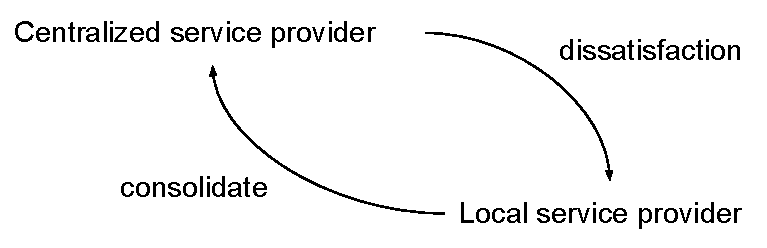
\includegraphics[width=0.8\textwidth]{images/dilemma_centralization-vs-distributed.pdf}
    \caption{Dipole oscillation. See Dilemma~\ref{table:central-vs-distributed}}
    \label{fig:central-vs-distributed}
\end{figure}

Centralization is often carried out for the purposes of cost efficiency. The cost savings are due to de-duplication and having less slack. Both of those ``savings'' are a decrease of redundancy, which has a cost when there are unexpected fluctuations in need. 

Centralization is an intentional monopolization, with the corresponding decrease in choices. 

Centralization (de-localization) can decrease the value assigned to feedback from people using the service because personal relations are de-valued. 

The weaker feedback, lack of redundancy, and decreased emphasis on relationships motivates the creation of local services. 

\ \\

\begin{center}
\begin{table}[ht]
\begin{tabular}{ | m{\dilemmatablewidth}| m{\dilemmatablewidth} | } 
  \hline
  \textbf{Decision making lower in a hierarchy} &
  \textbf{Decision making higher in a hierarchy} \\
  \hline
  \textit{Description}: Push decisions down to empower employees. &
  \textit{Description}: Escalate every decision to management. \\  
  \hline
  \textit{Pros}: better information &
  \textit{Pros}: better scope \\
  \hline
  \textit{Cons}: more inconsistency & 
  \textit{Cons}: Decision maker has less skin in the game and may be less well informed. Employees are disempowered. \\
  \hline
\end{tabular}
\caption{Where decisions get made in hierarchical organization.
%{\tiny Tag: Design of organization.}
}
\label{table:decisions_low-vs-high}
\end{table}
\end{center}

\ \\

\begin{center}
\begin{table}[ht]
\begin{tabular}{ | m{\dilemmatablewidth}| m{\dilemmatablewidth} | } 
  \hline
  \textbf{Redundant services in a market} &
  \textbf{Monopoly service provider} \\
  \hline
  \textit{Description}: using a market model within the organization &
  \textit{Description}:  \\  
  \hline
  \textit{Pros}: enable customers to choose the best service &
  \textit{Pros}: efficiency of a single service \\
  \hline
  \textit{Cons}: redundancy & 
  \textit{Cons}: might not meet the needs of all customers \\
  \hline
\end{tabular}
\caption{Services within an organization. See also Fig.~\ref{fig:market-vs-monopoly}.
%{\tiny Tag: Design of organization.}
}
\label{table:market-vs-monopoly}
\end{table}
\end{center}


\begin{figure}[ht]
    \centering
    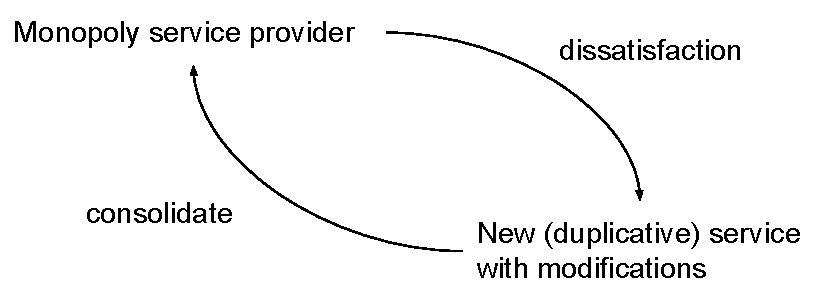
\includegraphics[width=0.8\textwidth]{images/dilemma_market_vs_monopoly.pdf}
    \caption{Dipole oscillation: solution A exists but doesn't meet my needs. Rather than tweak A, re-invent solution B which mostly overlaps with A but has independent development and support. See also Dilemma~\ref{table:market-vs-monopoly}.}
    \label{fig:market-vs-monopoly}
\end{figure}


% https://graphthinking.blogspot.com/2021/04/laffer-curve-and-minimum-viable.html
Goldilocks situation for amount of processes:
* too few processes (all social relationships)
* just the right amount -- a balance process and social, and when to use which is known.
* too much process (not enough leveraging of social relationships)
Similar to the \href{https://en.wikipedia.org/wiki/Laffer_curve}{Laffer curve} in economics.



% https://graphthinking.blogspot.com/2021/12/hierarchical-organization-trilemma.html
Trilemma: \textbf{Do you work for your team, your manager, or yourself?}
Being a member of a team that operates within a hierarchy is tough. One reason is the question of who you are working for. The trilemma is whether you work for yourself, work for your supervisor, or work for your team.  Ideally you can find ways to do all three, but that is not always the case. 

Members of the team should work collaboratively, but there is a potential counter-force: accountability to the supervisor. Because each team member is accountable to their supervisor(s), that motivates the action of the individual. The team does not actually have autonomy -- they are accountable to the boss.

In the approach ``team members are directed by their supervisor," the synergy of the team is neglected and the supervisor becomes a bottleneck (for decision making and for creativity and for planning).

The third approach is for a person to ignore their team and their supervisor. This might enable quicker progress, at the risk of going in an unhelpful direction or not leveraging skills of coworkers. 

\ \\

Trilemma:
Seek less budget, same, or larger budget 

\ \\

A trilemma applicable to many situations is that options are \textbf{fast, inexpensive, good; choose two}. (This is the \href{https://en.wikipedia.org/wiki/Project_management_triangle}{Project management triangle}.) \\
In other words, the options are
\begin{itemize}
    \item good and fast is expensive (i.e., requires lots of resources)
    \item good and inexpensive takes a long time (i.e., a clever solution)
    \item fast and inexpensive will be low quality
\end{itemize}

\ \\

There are many of dilemmas. Even if everyone considers the same choices (which doesn't necessarily happen), not everyone makes the same selection. Is the right response to defer to someone higher in the hierarchy to coordinate? While this would ensure consistency, this would be micromanagement. The people in the hierarchy above the person facing the choice don't have exposure to the problem.


Three ``so what" for dilemmas/trilemmas:
1) construct pareto frontier to identify non-optimal choices that can be eliminated
2) instead of assess variables in isolation, assess in workflows
3) raise subjective decisions to explicit discussion with stakeholders so that disagreement can be negotiated .


